\chapter{Physics Background} \label{ch:background}

% \section{Quantum Chromodynamics}

% \section{Phase Transitions}

% \section{Quark-Gluon Plasma}

% \section{Relativistic Heavy Ion Collisions}
% \subsection{RHIC and LHC}
% \subsection{Collision Energy, Centrality and Participants}
% \subsection{QGP Evolution}
% \subsection{Detection of Collision Products}
% \subsubsection{Tracking Detectors}
% \subsubsection{Calorimeters}

% \section{Detection of QGP Signatures}
% \subsection{Bjorken Energy Density}
% \subsection{Collective Flow}
% \subsection{Strangeness Enhancement}
% \subsection{Jet Quenching}
% \subsection{Photon Production}
% \section{Transverse Energy}
% \section{RHIC Beam Energy Scan Program}

\section{Quantum Chromodynamics}\label{section:QCD}
The strong force is one of the four fundamental interactions in physics. At large scale, it is responsible for binding the nucleons together to give the nucleus its structure. At the smaller scale, it binds the fundamental units of subnuclear matter, the quarks, together to form the nucleons. The electrodynamic interaction between charged particles such as protons and electrons is described by quantum electrodynamics (QED) as mediated by photons; the strong interaction, albeit more complicated, is explained under the framework of quantum chromodynamics (QCD) as mediated by gluons. \cite{KAPUSTA1979461, Shuryak1988} ???? The quarks and gluons of QCD are collectively known as partons.

%Along with electric charge, mass and spin, quarks have the intrinsic property of color charge. 
One of the phenomenological aspects in which QCD is different from QED is the confinement of partons. In QED, the fundamental particles are bound together by the Coulomb potential, which diminishes with distance between the charge-carrying particles, as demonstrated by the relation \ref{eqn:QED-potential}:
\begin{equation}\label{eqn:QED-potential}
V_{C}\propto\frac{1}{r} 
\end{equation}
where $V_{C}$ is the Coulomb potential, and $r$ is the spatial separation between the particles. This means that bound QED particles can be isolated by increasing their spatial separation. The QCD potential, on the other hand, has an extra linear term in it:
\begin{equation}\label{eqn:QCD-potential}
V_{QCD} = -\frac{4}{3}\frac{\alpha_{S}}{r} + {k}{r} 
\end{equation}
%(pg 7 https://www2.ph.ed.ac.uk/~muheim/teaching/np3/lect-qcd.pdf)
where $\alpha_{S}$ is the QCD fine-structure constant and k is is the strengh of the color interaction ($~$1 GeV/fm). This means that the potential increases linearly with distance at large distances, and so an infinite amount of energy is required to separate quarks. Hence, we never observe isolated quarks and they are said to be confined, not just bound, to form composite structures called hadrons.\cite{0954-3899-32-3-R01} Composition of a quark and an anti-quark forms a meson and that of three quarks forms a baryon.
%These confined, bound states of quarks and gluons is color-neutral.
%, and it is ergonomically more favorable to create a quark-antiquark pair than to produce unbound quarks
%, and $\alpha\_{QED}$ is the coupling constant.

\section{Phase Transitions}
In everyday life, we observe matter existing in four distinct phases: solid, liquid, gas, and plasma. Changes in physical conditions can lead to a transition from one of these phases to another, exemplified by the commonly observed coversion of ice to water. Distinctions among the various phases can be represented in a chart called the phase diagram.

The phase diagram consists of thermodynamic observables such as temperature and density on its axes. Curves in the phase diagram represent boundries of physical conditions at which two or more phases of matter can coexist in equilibrium. Crossing a boundary represents an abrupt transition from one phase to another; this abruptness is mathematically characterized by the discontinuity in the change of the derivative of the free energy -- a thermodynamic varible -- with respect to the physical quantities in the axes. There can also be regions in the diagram representing the ranges of physical conditions in which a smooth phase transition can take place.

One of the main focuses of current experimental and theoretical nuclear physics research is the study of the phase diagram of strongly interacting matter at a range of temperatures and baryon chemical potentials. In experiments involving the collisions of heavy ions at high and low energies, different regions of the phase diagram can be probed by varying the collision energy \cite{PhysRevC.93.024901}. For instance, the high-baryon chemical potential regime corresponds to lower beam energies and higher temperatures correspond to higher beam energies. The results of these experiments and model calculations can be used to study the nature of transitions in the QCD phase diagram.

A schematic representing the QCD phase diagram on the temperature (T) and quark chemical potential ($\mu$) plane is shown in Figure \ref{fig:PhaseDiagram} \cite{1742-6596-761-1-012066}. A second-order transition is predicted at low baryon chemical potentials (close to baryon-antibaryon symmetry) and high temperatures reminiscent of the early universe. Methods to study this region of the phase space will be explored in this thesis. At low temperatures and high chemical potentials, loose predictions have been made regarding the existence of exotic phases of high density matter, and programs, such as the Compressed Baryonic Matter experiment at the Facility for Antiproton and Ion Research in Germany, are being designed to study this region of the phase diagram.
% but within reach at modern facilities, specifically the Relativistic Heavy Ion Collider (RHIC) at the Brookhaven National Laboratory and the Large Hadron Collider (LHC) at CERN
%Details about these facilities are given in \ref{section:RHI-collisions}.
\begin{figure}[h]
  \centering
  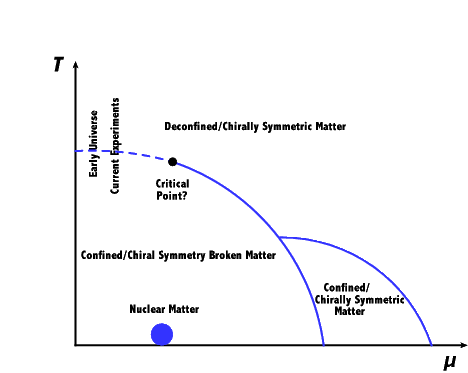
\includegraphics[width=5.5in]{figures/1742-6596-761-1-012066.png}\\
  \caption{Schematic of the QCD phase diagram \cite{1742-6596-761-1-012066}.}\label{fig:PhaseDiagram}
\end{figure}


\section{Quark-Gluon Plasma}
The confinement of quarks into the hardonic phase of QCD matter, as described in section \ref{section:QCD}, has its limitations. At very high densities, when the wave function of a single hadron encompasses the spatial regions covered by multiple such hadrons, it is impossible to classify which pair or triplet of quarks belongs to which meson or baryon. As long as a particular quark is close enough to the other quarks in the volume, it is deconfined in such a way that it can freely move anywhere in the volume. \cite{0954-3899-32-3-R01} QCD predicts a phase transition, at energy densities above 0.2-1 GeV/fm$^{3}$ \cite{Adam:2139456} and around a critical temperature of about 200 MeV \cite{2013arXiv1304.1452M}, of strongly interacting matter to a phase with quarks and gluons in thermal and chemical equilibrium representing the relevant degrees of freedom and behaving like an almost perfect quantum fluid \cite{PhysRevLett.109.152303}. This deconfined state of quarks and gluons is termed the quark-gluon plasma (QGP) in analogy to the quantum electrodynamical plasma phase of matter.

%The deconfinement is what the weakening of the strong interaction due to the polarization of the QCD vacuum is expected to lead to at high energies. The expectation of this phase transition also makes sense in terms of the chiral symmetry of the QCD Lagrangian, which is spontaneously broken at low temperatures, but restored at high temperatures, providing a sufficient condition for the deconfinement.
% Existence of QGP in the early universe
% Production of QGP in the lab

\section{Relativistic Heavy Ion Collisions}\label{section:RHI-collisions}
The experimental evidences of the theoretically appealing existence of QGP come from the collisions of large nuclei. The signatures of such evidence are described in section \ref{subsection:detection}. Physicists started noting down such evidences since as far back as 1984, when nuclei were accelerated and collided with stationary targets.\cite{Gyulassy:2004vg} They were able to agree on a conclusive discovery of this matter during the 2000s, after colliding accelerated nuclei with other such nuclei or smaller species (protons, deuterons) at unprecedented energies and with improved detection schemes. \cite{Ritter:2004xj} With further increase in collision energies and enhancement in detector technololgy, modern accelerator facilities have not only added such evidences but also provided estimates of some of the properties as well as the dynamics of the evolution of the QGP. The following subsections describe two such facilities, the physics of the collisions and what happens after the collisions.
\subsection{RHIC and LHC}

\subsection{Collision Energy, Centrality and Participants}
\subsection{QGP Evolution}
\subsection{Detection of Collision Products}\label{subsection:detection}
\subsubsection{Tracking Detectors}
\subsubsection{Calorimeters}

\section{Detection of QGP Signatures}
http://iopscience.iop.org/article/10.1088/0954-3899/25/3/013/meta, and: 

The existence and properties of the QGP in the aftermath of high-energy heavy-ion collisions can be probed using different techniques relevant to several theoretical characteristics of the phase. For instance, the interacting nuclei  carry no net strangeness before colliding, and so a post-collision observation of strange and multi-strange particles can be a signal for an antecedent existence of deconfined quarks and gluons \cite{1742-6596-455-1-012005}. This signal, when complemented with an observation of the suppression???????or enhancement of strange particles production, provides a strong hint of the formation of QGP. This can be further complemented with the estimate of the energy density and the temperature attained after the collision.

Analyses of experimental results have thus far provided signatures of the formation of matter with partonic degrees of freedom at the early stages of the collisions. Such signatures include suppression of high monentum hadrons, known as jet quenching, because the QGP is nearly opaque to colored probes, and large azimuthal anisotropies, indicating that the medium is a liquid of quarks and gluons \cite{PhysRevC.96.044904}?????. Experiments also reveal the initial energy density of this matter to be about two orders of magnitude larger than that of low energy nuclear matter -- comfortably more than the deconfinement phase transition critical density predicted by lattice QCD \cite{2005PrPNP..54..443J}.

The state of the colliding nuclei before the collision at LHC and top RHIC energies has indications of being a Color Glass Condensate -- strongly interacting, weakly coupled highly coherent gluonic matter \cite{1742-6596-458-1-012024}. The characteristics of the initial states of these nuclei affect the partonic distributions within the nuclei and ultimately the products of the collision. The collision products are also affected by variables such as the initial energy and entropy densities of the partonic matter \cite{2005PrPNP..54..443J}.

Different observables can be used to study different aspects of heavy ion collisions. The charged particle multiplicity, $\langle N_{ch} \rangle$, is a global variable that relates to the entropy production during the collision (analysis note). The transverse energy, $E_{T}$, a global variable related to $\langle N_{ch} \rangle$, provides information about the conversion of the initial beam-direction kinetic energy into energy flowing in the transverse direction after the collision. Together, the studies of the fluctuation of the $\langle N_{ch} \rangle$ and the $E_{T}$ pseudorapidity [footnote] density with respect to the beam energy and the collision centrality [footnote] help probe the characteristics of the initial conditions at the time of the collision. One can study, for instance, the distinctions between models based on quark participants against those based on nucleon participants [analysis note]. These quantities can also lead to the rough estimate of the initial energy density through the use of the Bjorken formula \cite{2012ARNPS..62..361M}:
%\ref{eqn:Bjorken}
\begin{equation}\label{eqn:Bjorken}
\epsilon \geq \frac{\frac{dE_{T}}{d\eta}}{\tau_{0}\pi R^{2}} = \frac{3}{2}\langle \frac{E_{T}}{N} \rangle \frac{\frac{dN_{ch}}{d\eta}}{\tau_{0}\pi R^{2}}
\end{equation}

The transverse energy and the charged particle pseudorapidity densities have conventionally been calculated by using the transverse energy measurements obtained from calorimeters. This thesis details the use of particle spectra, reported as $\frac{d^{2}N}{dydp_{T}}$, from Au+Au collisions at RHIC to calculate the same global variables and serve as a method to cross check the ones involving calorimeters.
\subsection{Bjorken Energy Density}
\subsection{Collective Flow}
\subsection{Strangeness Enhancement}
\subsection{Jet Quenching}
\subsection{Photon Production}
Why does large elliptic flow suggest large rescattering among partons and early thermalization of high pT partons? 
\section{Transverse Energy}
\section{RHIC Beam Energy Scan Program}
